\subsection{Realizzazione}
Dopo aver tenuto conto di alcuni accorgimenti come l'inserimento di consensatori
per il disaccoppiamento e i terminali necessari per collegarsi agli altri
circuiti è stato disegnato un PCB non definitivo ma utile come riferimento per
la realizzazione del circuito su scheda millefori.

\begin{figure}[H]
    \centering
    \begin{subfigure}{0.49\textwidth}
        \centering
        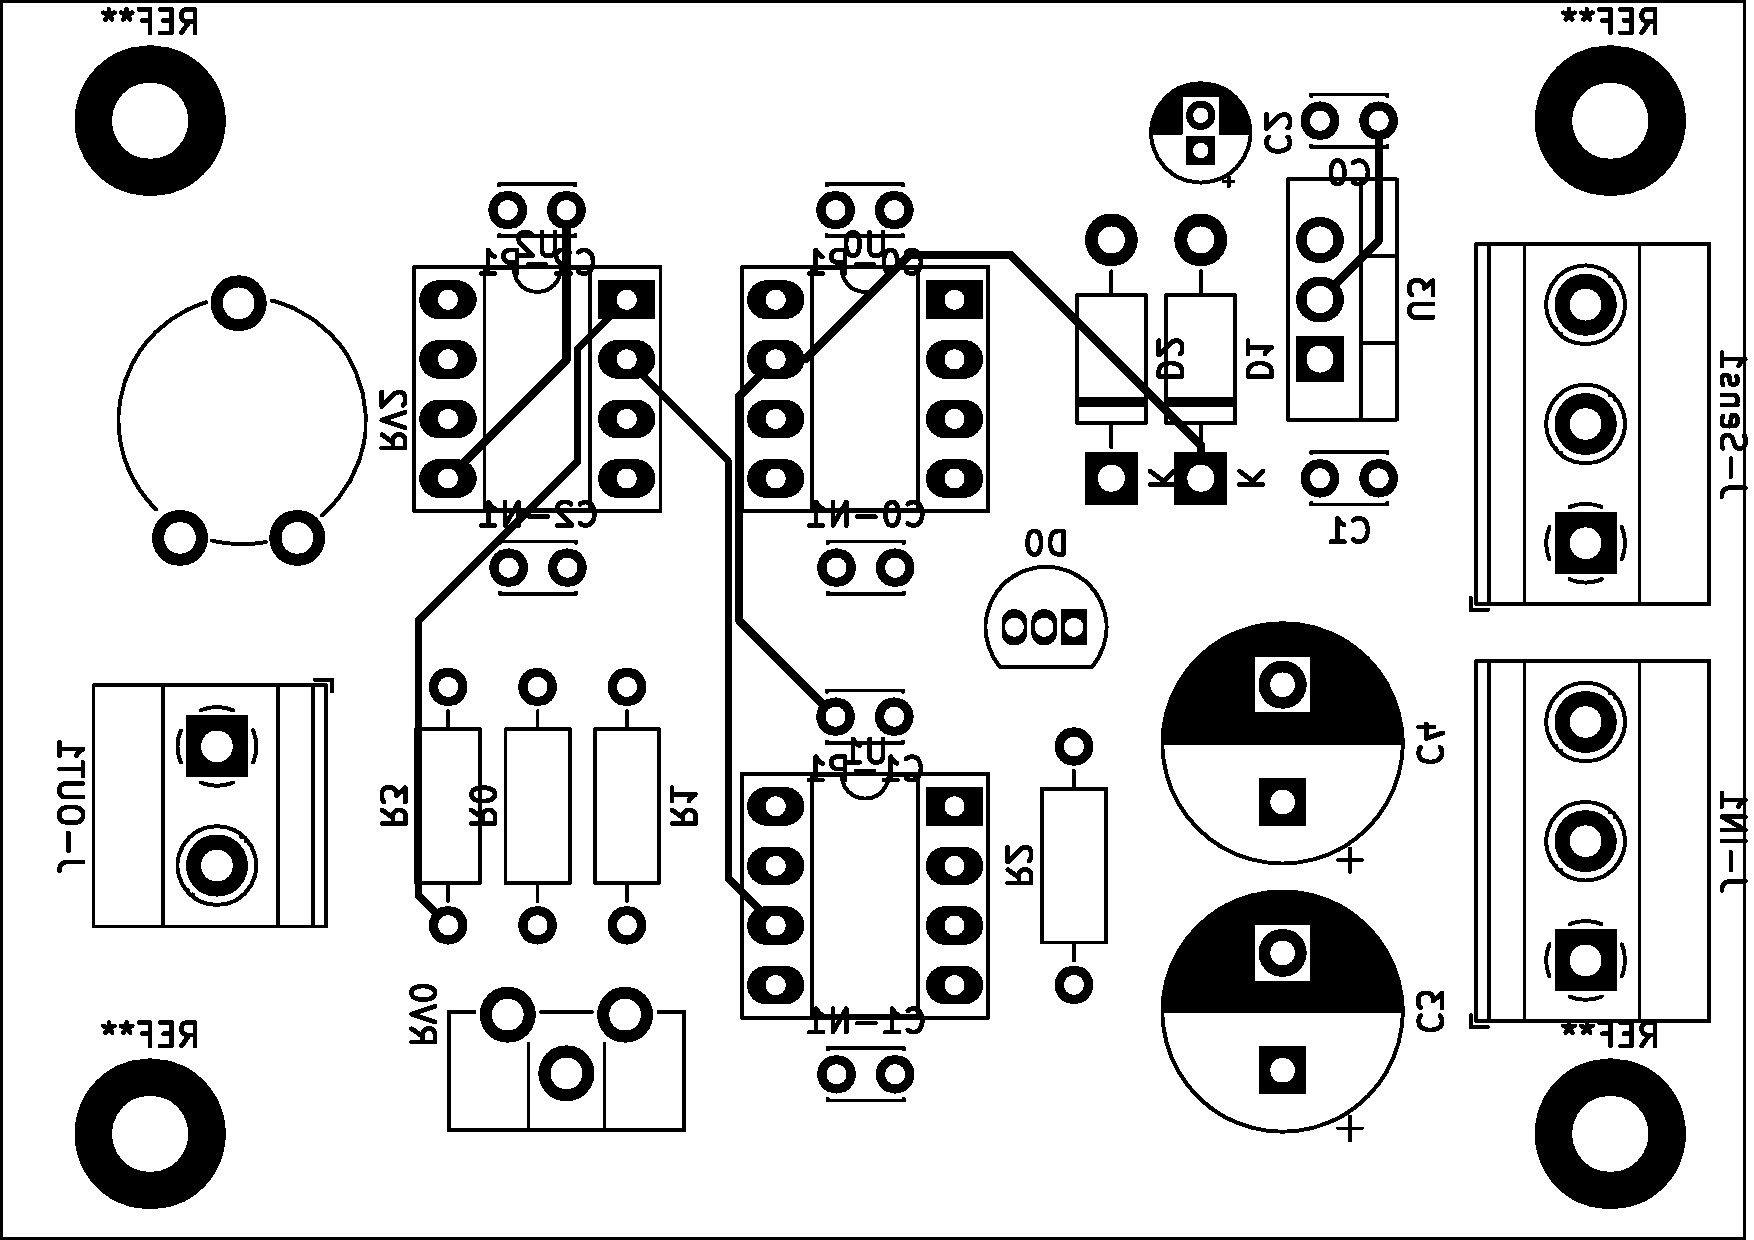
\includegraphics[scale=0.25]{corrente/top.pdf}
        \caption{Stampa Copper Top}
    \end{subfigure}
    \begin{subfigure}{0.49\textwidth}
        \centering
        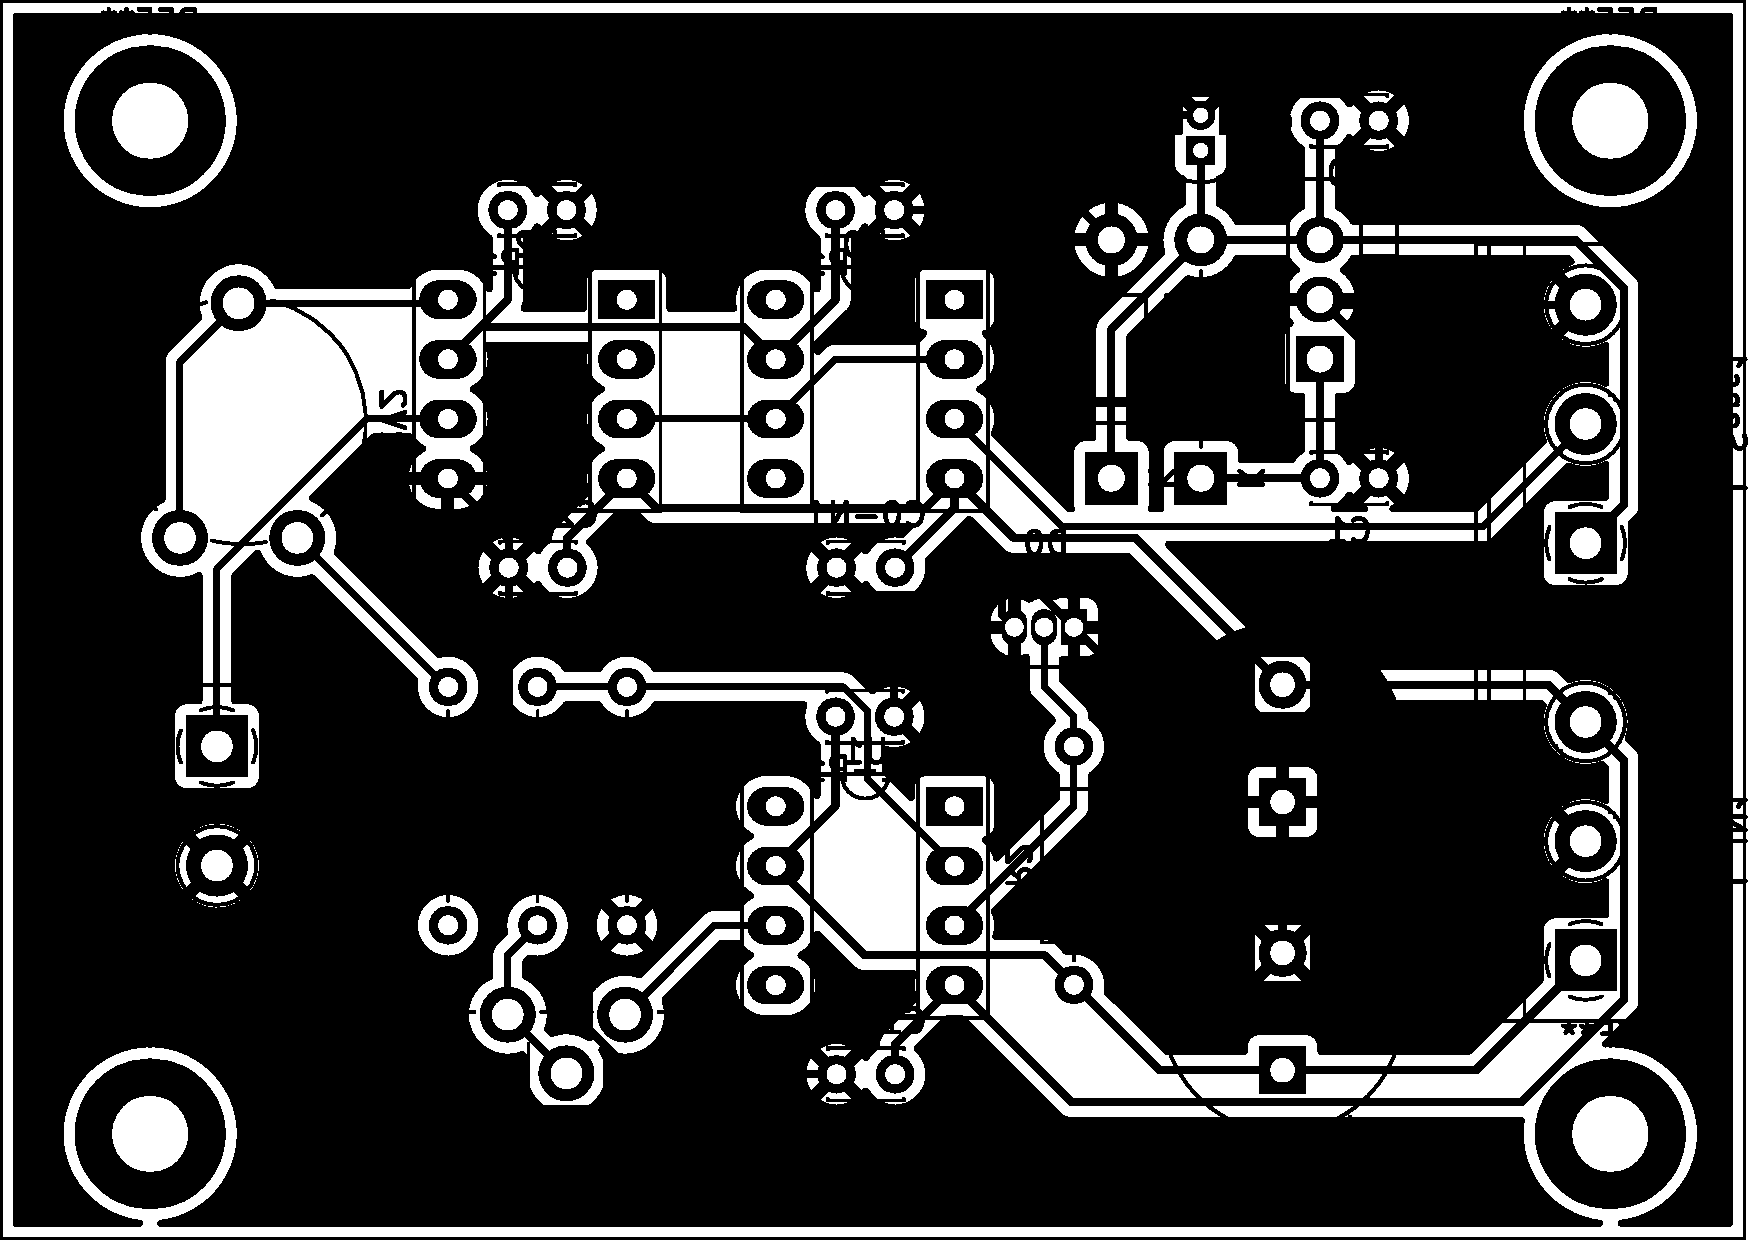
\includegraphics[scale=0.25]{corrente/bottom.pdf}
        \caption{stampa Copper Bottom}
    \end{subfigure}
    \caption{Stampe piste e serigrafia}
\end{figure}

%%AGGIUNGERE STAMPE 3D

\subsection{Taratura}